\documentclass{article}\usepackage[]{graphicx}\usepackage[]{xcolor}
% maxwidth is the original width if it is less than linewidth
% otherwise use linewidth (to make sure the graphics do not exceed the margin)
\makeatletter
\def\maxwidth{ %
  \ifdim\Gin@nat@width>\linewidth
    \linewidth
  \else
    \Gin@nat@width
  \fi
}
\makeatother

\definecolor{fgcolor}{rgb}{0.345, 0.345, 0.345}
\newcommand{\hlnum}[1]{\textcolor[rgb]{0.686,0.059,0.569}{#1}}%
\newcommand{\hlsng}[1]{\textcolor[rgb]{0.192,0.494,0.8}{#1}}%
\newcommand{\hlcom}[1]{\textcolor[rgb]{0.678,0.584,0.686}{\textit{#1}}}%
\newcommand{\hlopt}[1]{\textcolor[rgb]{0,0,0}{#1}}%
\newcommand{\hldef}[1]{\textcolor[rgb]{0.345,0.345,0.345}{#1}}%
\newcommand{\hlkwa}[1]{\textcolor[rgb]{0.161,0.373,0.58}{\textbf{#1}}}%
\newcommand{\hlkwb}[1]{\textcolor[rgb]{0.69,0.353,0.396}{#1}}%
\newcommand{\hlkwc}[1]{\textcolor[rgb]{0.333,0.667,0.333}{#1}}%
\newcommand{\hlkwd}[1]{\textcolor[rgb]{0.737,0.353,0.396}{\textbf{#1}}}%
\let\hlipl\hlkwb

\usepackage{framed}
\makeatletter
\newenvironment{kframe}{%
 \def\at@end@of@kframe{}%
 \ifinner\ifhmode%
  \def\at@end@of@kframe{\end{minipage}}%
  \begin{minipage}{\columnwidth}%
 \fi\fi%
 \def\FrameCommand##1{\hskip\@totalleftmargin \hskip-\fboxsep
 \colorbox{shadecolor}{##1}\hskip-\fboxsep
     % There is no \\@totalrightmargin, so:
     \hskip-\linewidth \hskip-\@totalleftmargin \hskip\columnwidth}%
 \MakeFramed {\advance\hsize-\width
   \@totalleftmargin\z@ \linewidth\hsize
   \@setminipage}}%
 {\par\unskip\endMakeFramed%
 \at@end@of@kframe}
\makeatother

\definecolor{shadecolor}{rgb}{.97, .97, .97}
\definecolor{messagecolor}{rgb}{0, 0, 0}
\definecolor{warningcolor}{rgb}{1, 0, 1}
\definecolor{errorcolor}{rgb}{1, 0, 0}
\newenvironment{knitrout}{}{} % an empty environment to be redefined in TeX

\usepackage{alltt}
\usepackage[margin=1.0in]{geometry} % To set margins
\usepackage{amsmath}  % This allows me to use the align functionality.
                      % If you find yourself trying to replicate
                      % something you found online, ensure you're
                      % loading the necessary packages!
\usepackage{amsfonts} % Math font
\usepackage{fancyvrb}
\usepackage{hyperref} % For including hyperlinks
\usepackage[shortlabels]{enumitem}% For enumerated lists with labels specified
                                  % We had to run tlmgr_install("enumitem") in R
\usepackage{float}    % For telling R where to put a table/figure
\usepackage{natbib}        %For the bibliography
\bibliographystyle{apalike}%For the bibliography
\IfFileExists{upquote.sty}{\usepackage{upquote}}{}
\begin{document}

In lecture 16, we looked at precipitation amounts in Madison County (at 
Morrisville station). We found that the Weibull distribution had a good fit
to the monthly precipitation amounts.\\

We found that the MLEs for the Weibull distribution were 
\begin{align*}
    \hat{a}&=2.1871\\
    \hat{\sigma}&=3.9683
\end{align*}
and
\[-\mathcal{L}(\{\hat{a}, \hat{\sigma}\}|\mathbf{x}) = 2166.496\]
is the realized negative log-likelihood.
Note this means that the log-likelihood is
\[\mathcal{L}(\{\hat{a}, \hat{\sigma}\}|\mathbf{x}) = -2166.496,\]
and the usual likelihood is
\[L(\{\hat{a}, \hat{\sigma}\}|\mathbf{x}) = e^{\left[\mathcal{L}(\{\hat{a}, \hat{\sigma}\}|\mathbf{x})\right]} \approx = e^{-2166.496},\]
which \texttt{R} cannot differentiate from 0.

\begin{enumerate}
  \item Someone asked ``why Weibull?" in class. That is, why wouldn't we use 
  another right-skewed distribution like the Gamma (see Lecture 15), or
  the Log-Normal (see Lecture 17).
  \begin{enumerate}
    \item Compute the MLEs for these data using a Gamma distribution.

\textbf{Solution:} The computed MLEs for these data using the gamma distribution turned out to be \[\hat{\alpha}=4.17, \hat{\beta}=1.19\]
    
    \item Compute the MLEs for these data using the Log-Normal distribution.
    
  \textbf{Solution:} The computed MLEs for these data using the gamma distribution turned out to be \[\hat{\mu}=1.131, \hat{\sigma}=0.533\]
    
    \item Compute the likelihood ratio to compare the Weibull and the Gamma distribution. 
    Which has a better fit according to the likelhiood ratio?
  \\
  \textbf{Solution:} Since the likelihood ratio is greater than 1 that means that the Weibull distribution is a better fit for the data than the Gamma distribution.
    \[Q = \frac{L(\{\hat{a}, \hat{\sigma}\}|\mathbf{x})}{L(\{\hat{\alpha}, \hat{\beta}\}|\mathbf{x})}=e^{\left[\mathcal{L}(\{\hat{a}, \hat{\sigma}\}|\mathbf{x}) - \mathcal{L}(\{\hat{\alpha}, \hat{\beta}\}|\mathbf{x})\right]}=1.0071\]
    \item Compute the likelihood ratio to compare the Weibull and the Log-Normal distribution.
    Which has a better fit according to the likelihood ratio?
    \\
    \textbf{Solution:} Since the likelihood ratio is less than 1 that means that the Log-Normal distribution is a better fit for the data than the Weibull distribution.
    \\
    \[Q = \frac{L(\{\hat{a}, \hat{\sigma}\}|\mathbf{x})}{L(\{\hat{\mu}, \hat{\sigma}\}|\mathbf{x})}=e^{\left[\mathcal{L}(\{\hat{a}, \hat{\sigma}\}|\mathbf{x}) - \mathcal{L}(\{\hat{\mu}, \hat{\sigma}\}|\mathbf{x})\right]}=0.9828\]
    \item Compute the likelihood ratio to compare the Gamma and the Log-Normal distribution.
    Which has a better fit according to the likelhiood ratio?
    \\
    \textbf{Solution:} Since the likelihood ratio is less than 1 that means that the Log-Normal distribution is a better fit for the data than the Gamma distribution.
    \\
    \[Q = \frac{L(\{\hat{\alpha}, \hat{\beta}\}|\mathbf{x})}{L(\{\hat{\mu}, \hat{\sigma}\}|\mathbf{x})}=e^{\left[\mathcal{L}(\{\hat{\alpha}, \hat{\beta}\}|\mathbf{x}) - \mathcal{L}(\{\hat{\mu}, \hat{\sigma}\}|\mathbf{x})\right]}=0.9759\]
  \end{enumerate}
  \item \textbf{CODE:}
  \\
\begin{knitrout}
\definecolor{shadecolor}{rgb}{0.969, 0.969, 0.969}\color{fgcolor}\begin{kframe}
\begin{alltt}
\hlkwd{library}\hldef{(tidyverse)}
\hlkwd{library}\hldef{(nleqslv)}
\hlkwd{library}\hldef{(patchwork)}

\hldef{dat} \hlkwb{=} \hlkwd{read_csv}\hldef{(}\hlsng{"agacis.csv"}\hldef{)}

\hldef{dat.long} \hlkwb{<-} \hldef{dat |>}
  \hldef{dplyr}\hlopt{::}\hlkwd{select}\hldef{(}\hlopt{-}\hldef{Annual) |>}                   \hlcom{# Remove annual column }
  \hlkwd{pivot_longer}\hldef{(}\hlkwc{cols} \hldef{=} \hlkwd{c}\hldef{(Jan, Feb, Mar, Apr,}   \hlcom{# pivot the column data into one col}
                        \hldef{May, Jun, Jul, Aug,}
                        \hldef{Sep, Oct, Nov, Dec),}
               \hlkwc{values_to} \hldef{=} \hlsng{"Precipitation"}\hldef{,}   \hlcom{# store the values in Precipitation}
               \hlkwc{names_to} \hldef{=} \hlsng{"Month"}\hldef{) |>}         \hlcom{# store the months in Month}
  \hlkwd{mutate}\hldef{(}\hlkwc{Precipitation} \hldef{=} \hlkwd{case_when}\hldef{(Precipitation} \hlopt{==} \hlsng{"M"} \hlopt{~} \hlnum{NA_character_}\hldef{,}
                                   \hlnum{TRUE}                 \hlopt{~} \hldef{Precipitation))|>}
  \hlkwd{mutate}\hldef{(}\hlkwc{Precipitation} \hldef{=} \hlkwd{as.numeric}\hldef{(Precipitation))}

\hlcom{### Weibull}
\hldef{llweibull} \hlkwb{<-} \hlkwa{function}\hldef{(}\hlkwc{par}\hldef{,} \hlkwc{data}\hldef{,} \hlkwc{neg}\hldef{=F)\{}
  \hlcom{# a <- par[1]}
  \hlcom{# sigma <- par[2]}
  \hldef{a} \hlkwb{<-} \hlkwd{exp}\hldef{(par[}\hlnum{1}\hldef{])} \hlcom{# go from (-inf,inf) to (0,inf)}
  \hldef{sigma} \hlkwb{<-} \hlkwd{exp}\hldef{(par[}\hlnum{2}\hldef{])} \hlcom{# go from (-inf,inf) to (0,inf)}

  \hldef{ll} \hlkwb{<-} \hlkwd{sum}\hldef{(}\hlkwd{log}\hldef{(}\hlkwd{dweibull}\hldef{(}\hlkwc{x}\hldef{=data,} \hlkwc{shape}\hldef{=a,} \hlkwc{scale}\hldef{=sigma)),} \hlkwc{na.rm}\hldef{=T)}

  \hlkwd{return}\hldef{(}\hlkwd{ifelse}\hldef{(neg,} \hlopt{-}\hldef{ll, ll))}
\hldef{\}}

\hldef{weibulls} \hlkwb{=} \hlkwd{optim}\hldef{(}\hlkwc{fn} \hldef{= llweibull,}
              \hlkwc{par} \hldef{=} \hlkwd{c}\hldef{(}\hlnum{1}\hldef{,}\hlnum{1}\hldef{),}
              \hlkwc{data} \hldef{= dat.long}\hlopt{$}\hldef{Precipitation,}
              \hlkwc{neg}\hldef{=T)}

\hldef{weibull.a} \hlkwb{=} \hldef{weibulls}\hlopt{$}\hldef{par[}\hlnum{1}\hldef{]}
\hldef{weibull.sigma} \hlkwb{=} \hldef{weibulls}\hlopt{$}\hldef{par[}\hlnum{2}\hldef{]}

\hlcom{### Part A}
\hldef{gamma.MLE} \hlkwb{=} \hlkwa{function}\hldef{(}\hlkwc{data}\hldef{,} \hlkwc{par}\hldef{,} \hlkwc{neg}\hldef{=F)\{}
  \hldef{a} \hlkwb{=} \hldef{par[}\hlnum{1}\hldef{]}
  \hldef{b} \hlkwb{=} \hldef{par[}\hlnum{2}\hldef{]}

  \hldef{loglik} \hlkwb{<-} \hlkwd{sum}\hldef{(}\hlkwd{log}\hldef{(}\hlkwd{dgamma}\hldef{(}\hlkwc{x}\hldef{=data,} \hlkwc{shape} \hldef{= a,} \hlkwc{rate} \hldef{= b)),} \hlkwc{na.rm} \hldef{= T)}

  \hlkwd{return}\hldef{(}\hlkwd{ifelse}\hldef{(neg,} \hlopt{-}\hldef{loglik, loglik))}
\hldef{\}}

\hldef{gammas} \hlkwb{=} \hlkwd{optim}\hldef{(}\hlkwc{par} \hldef{=} \hlkwd{c}\hldef{(}\hlnum{1}\hldef{,} \hlnum{1}\hldef{),}
              \hlkwc{fn} \hldef{= gamma.MLE,}
              \hlkwc{data}\hldef{=dat.long}\hlopt{$}\hldef{Precipitation,}
              \hlkwc{neg}\hldef{=T)}

\hldef{gamma.a} \hlkwb{=} \hldef{gammas}\hlopt{$}\hldef{par[}\hlnum{1}\hldef{]}
\hldef{gamma.b} \hlkwb{=} \hldef{gammas}\hlopt{$}\hldef{par[}\hlnum{2}\hldef{]}

\hldef{dat.gamma} \hlkwb{<-} \hlkwd{tibble}\hldef{(}\hlkwc{x} \hldef{=} \hlkwd{seq}\hldef{(}\hlnum{0}\hldef{,}\hlnum{15}\hldef{,}\hlkwc{length.out}\hldef{=}\hlnum{1000}\hldef{)) |>}
  \hlkwd{mutate}\hldef{(}\hlkwc{pdf.mle} \hldef{=} \hlkwd{dgamma}\hldef{(}\hlkwc{x}\hldef{=x,} \hlkwc{shape}\hldef{=gammas}\hlopt{$}\hldef{par[}\hlnum{1}\hldef{],} \hlkwc{scale}\hldef{=gammas}\hlopt{$}\hldef{par[}\hlnum{2}\hldef{]))}

\hlkwd{ggplot}\hldef{()} \hlopt{+}
  \hlkwd{geom_histogram}\hldef{(}\hlkwc{data} \hldef{= dat.long,} \hlkwd{aes}\hldef{(}\hlkwc{x} \hldef{= Precipitation,} \hlkwc{y} \hldef{=} \hlkwd{after_stat}\hldef{(density)),}
  \hlkwc{breaks}\hldef{=}\hlkwd{seq}\hldef{(}\hlnum{0}\hldef{,} \hlnum{15}\hldef{,} \hlnum{1}\hldef{),}
  \hlkwc{color}\hldef{=}\hlsng{"grey"}\hldef{)}\hlopt{+}
  \hlkwd{geom_hline}\hldef{(}\hlkwc{yintercept} \hldef{=} \hlnum{0}\hldef{)}\hlopt{+}
  \hlkwd{geom_line}\hldef{(}\hlkwc{data} \hldef{= dat.gamma,} \hlkwd{aes}\hldef{(}\hlkwc{x} \hldef{= x,} \hlkwc{y} \hldef{= pdf.mle))}
\end{alltt}
\end{kframe}
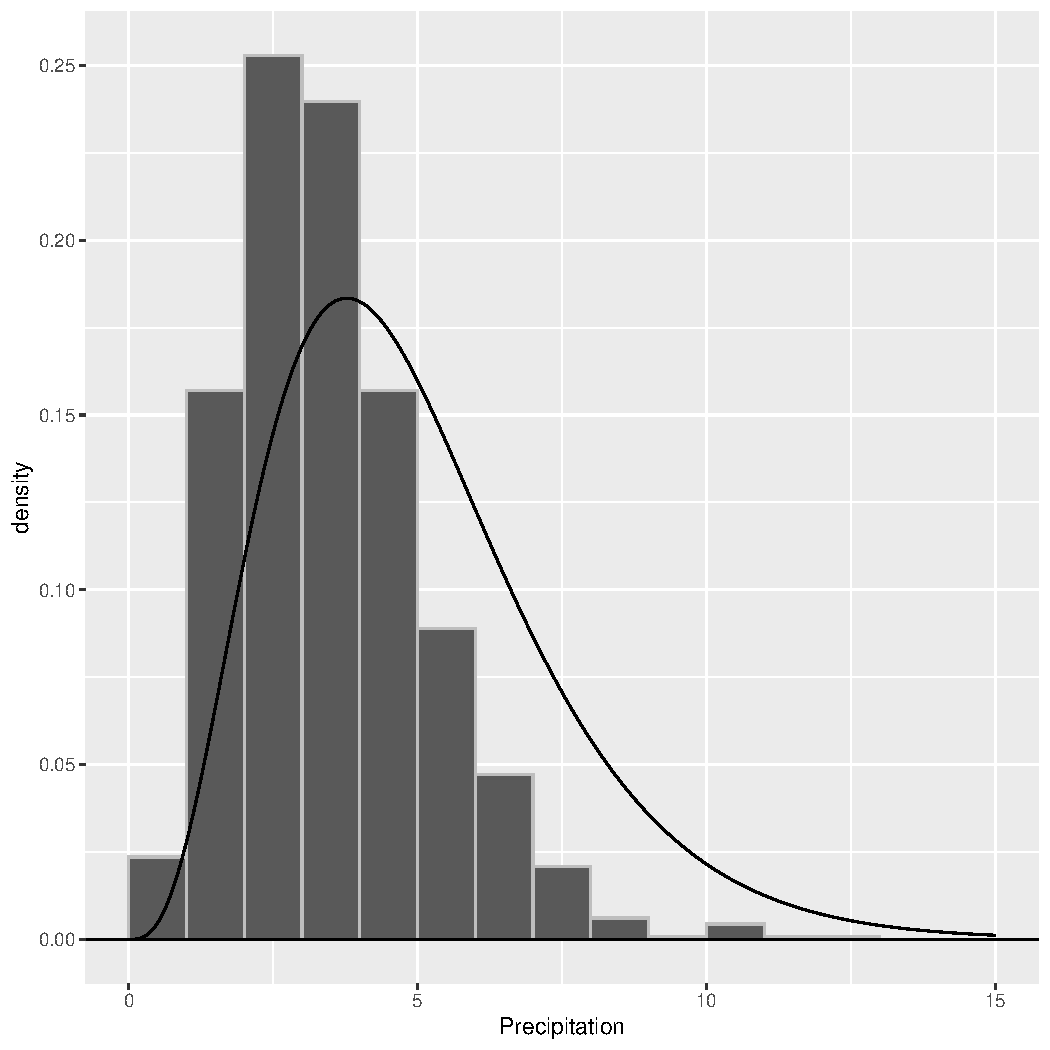
\includegraphics[width=\maxwidth]{figure/unnamed-chunk-2-1} 
\begin{kframe}\begin{alltt}
  \hlcom{###### PART B}
\hldef{lnorm.MLE} \hlkwb{=} \hlkwa{function}\hldef{(}\hlkwc{data}\hldef{,} \hlkwc{par}\hldef{,} \hlkwc{neg}\hldef{=F)\{}
  \hldef{mu} \hlkwb{=} \hldef{par[}\hlnum{1}\hldef{]}
  \hldef{sigma} \hlkwb{=} \hldef{par[}\hlnum{2}\hldef{]}

  \hldef{loglik} \hlkwb{<-} \hlkwd{sum}\hldef{(}\hlkwd{log}\hldef{(}\hlkwd{dlnorm}\hldef{(}\hlkwc{x}\hldef{=data,} \hlkwc{meanlog} \hldef{= mu,} \hlkwc{sdlog} \hldef{= sigma)),} \hlkwc{na.rm} \hldef{= T)}

  \hlkwd{return}\hldef{(}\hlkwd{ifelse}\hldef{(neg,} \hlopt{-}\hldef{loglik, loglik))}
\hldef{\}}

\hldef{lnorms} \hlkwb{=} \hlkwd{optim}\hldef{(}\hlkwc{par} \hldef{=} \hlkwd{c}\hldef{(}\hlnum{1}\hldef{,} \hlnum{1}\hldef{),}
              \hlkwc{fn} \hldef{= lnorm.MLE,}
              \hlkwc{data}\hldef{=dat.long}\hlopt{$}\hldef{Precipitation,}
              \hlkwc{neg}\hldef{=T)}

\hldef{lnorm.mu} \hlkwb{=} \hldef{lnorms}\hlopt{$}\hldef{par[}\hlnum{1}\hldef{]}
\hldef{lnorm.sd} \hlkwb{=} \hldef{lnorms}\hlopt{$}\hldef{par[}\hlnum{2}\hldef{]}

\hldef{dat.lnorm} \hlkwb{<-} \hlkwd{tibble}\hldef{(}\hlkwc{x} \hldef{=} \hlkwd{seq}\hldef{(}\hlnum{0}\hldef{,}\hlnum{15}\hldef{,}\hlkwc{length.out}\hldef{=}\hlnum{1000}\hldef{)) |>}
  \hlkwd{mutate}\hldef{(}\hlkwc{pdf.mle} \hldef{=} \hlkwd{dlnorm}\hldef{(}\hlkwc{x}\hldef{=x,} \hlkwc{meanlog}\hldef{=lnorms}\hlopt{$}\hldef{par[}\hlnum{1}\hldef{],} \hlkwc{sdlog}\hldef{=lnorms}\hlopt{$}\hldef{par[}\hlnum{2}\hldef{]))}



\hlkwd{ggplot}\hldef{()} \hlopt{+}
  \hlkwd{geom_histogram}\hldef{(}\hlkwc{data} \hldef{= dat.long,} \hlkwd{aes}\hldef{(}\hlkwc{x} \hldef{= Precipitation,} \hlkwc{y} \hldef{=} \hlkwd{after_stat}\hldef{(density)),}
                 \hlkwc{breaks}\hldef{=}\hlkwd{seq}\hldef{(}\hlnum{0}\hldef{,} \hlnum{15}\hldef{,} \hlnum{1}\hldef{),}
                 \hlkwc{color}\hldef{=}\hlsng{"grey"}\hldef{)}\hlopt{+}
  \hlkwd{geom_hline}\hldef{(}\hlkwc{yintercept} \hldef{=} \hlnum{0}\hldef{)}\hlopt{+}
  \hlkwd{geom_line}\hldef{(}\hlkwc{data} \hldef{= dat.lnorm,} \hlkwd{aes}\hldef{(}\hlkwc{x} \hldef{= x,} \hlkwc{y} \hldef{= pdf.mle))}
\end{alltt}
\end{kframe}
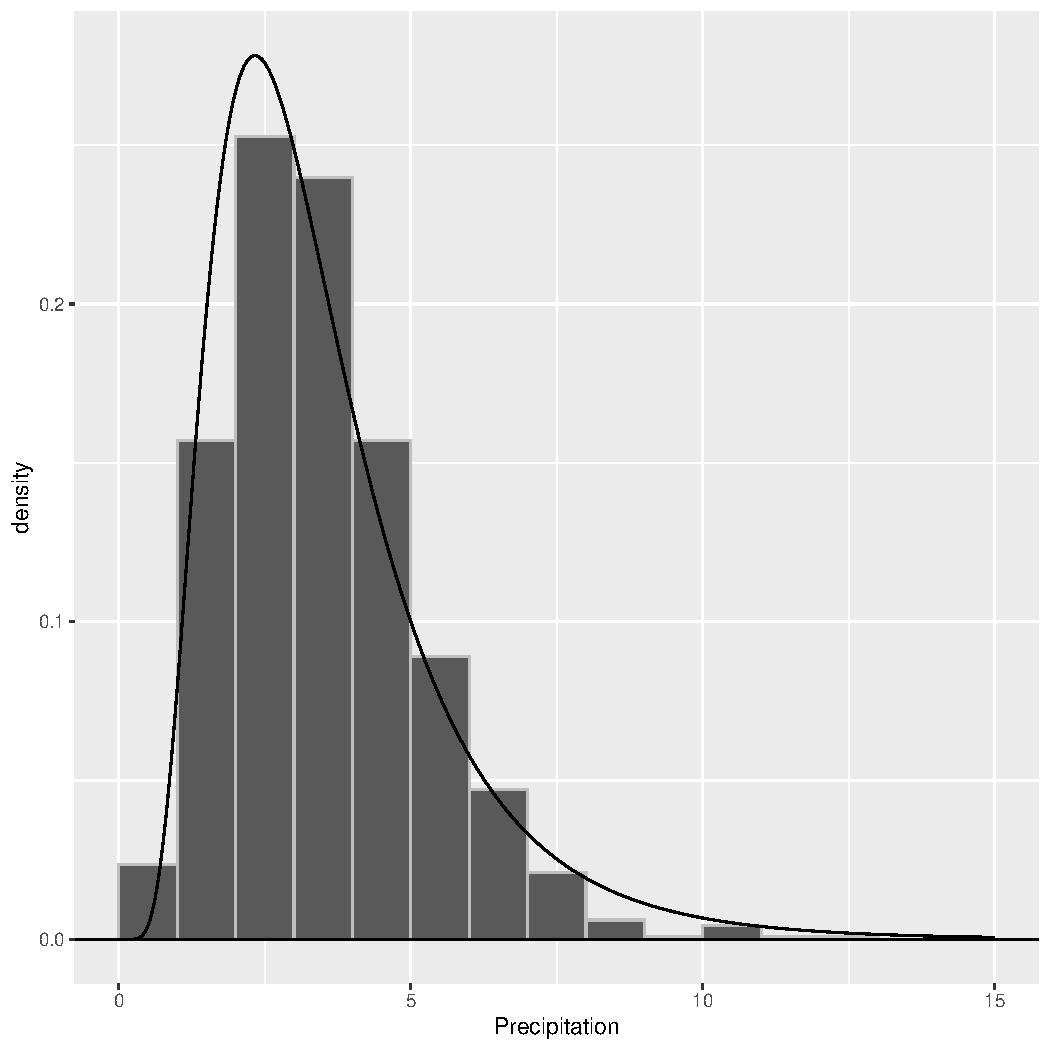
\includegraphics[width=\maxwidth]{figure/unnamed-chunk-2-2} 
\begin{kframe}\begin{alltt}
\hlcom{#### Part C}

\hldef{(weibull.gamma} \hlkwb{=} \hlkwd{llweibull}\hldef{(dat.long}\hlopt{$}\hldef{Precipitation,} \hlkwc{par} \hldef{= weibulls}\hlopt{$}\hldef{par)}
                \hlopt{/}\hlkwd{gamma.MLE}\hldef{(dat.long}\hlopt{$}\hldef{Precipitation,} \hlkwc{par} \hldef{= gammas}\hlopt{$}\hldef{par))}
\end{alltt}
\begin{verbatim}
[1] 1.007134
\end{verbatim}
\begin{alltt}
\hlcom{#### Part D}

\hldef{(weibull.lnorm} \hlkwb{=} \hlkwd{llweibull}\hldef{(dat.long}\hlopt{$}\hldef{Precipitation,} \hlkwc{par} \hldef{= weibulls}\hlopt{$}\hldef{par)}
  \hlopt{/}\hlkwd{lnorm.MLE}\hldef{(dat.long}\hlopt{$}\hldef{Precipitation,} \hlkwc{par} \hldef{= lnorms}\hlopt{$}\hldef{par))}
\end{alltt}
\begin{verbatim}
[1] 0.982894
\end{verbatim}
\begin{alltt}
\hlcom{#### Part E}

\hldef{(gamma.lnorm} \hlkwb{=} \hlkwd{gamma.MLE}\hldef{(dat.long}\hlopt{$}\hldef{Precipitation,} \hlkwc{par} \hldef{= gammas}\hlopt{$}\hldef{par)}
  \hlopt{/}\hlkwd{lnorm.MLE}\hldef{(dat.long}\hlopt{$}\hldef{Precipitation,} \hlkwc{par} \hldef{= lnorms}\hlopt{$}\hldef{par))}
\end{alltt}
\begin{verbatim}
[1] 0.9759315
\end{verbatim}
\end{kframe}
\end{knitrout}
  
\end{enumerate}

\bibliography{bibliography}
\end{document}
